\begin{figure*}[t!]
    \centering
    \begin{subfigure}[b]{0.3\textwidth}
    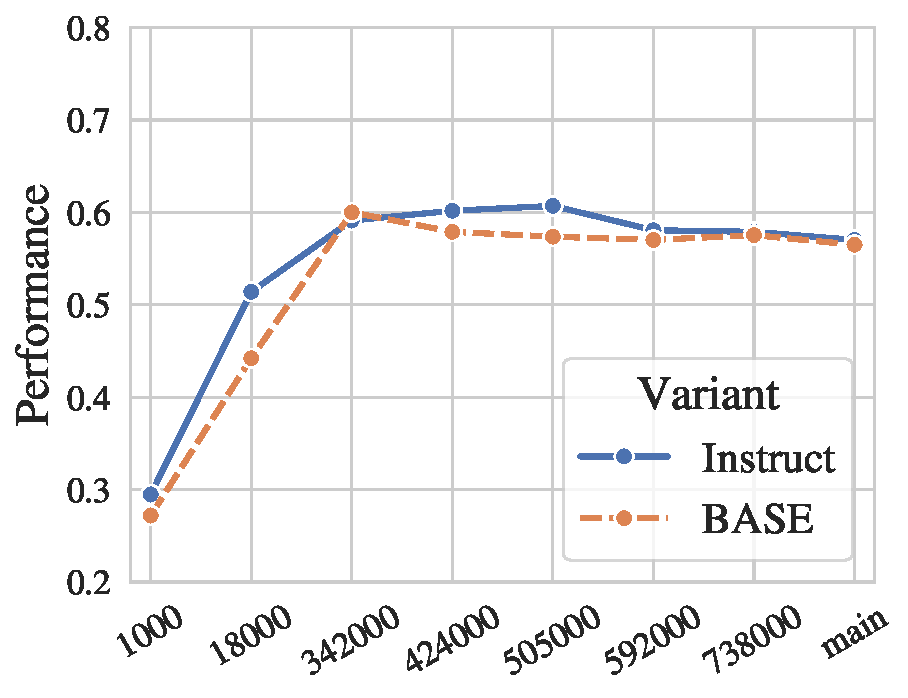
\includegraphics[width=\the\columnwidth]{figures/fig_files/it_ckpts/it_evalarc_easy.pdf}
        \caption{ARC Easy}
    \end{subfigure}%
    ~ 
    \begin{subfigure}[b]{0.3\textwidth}
    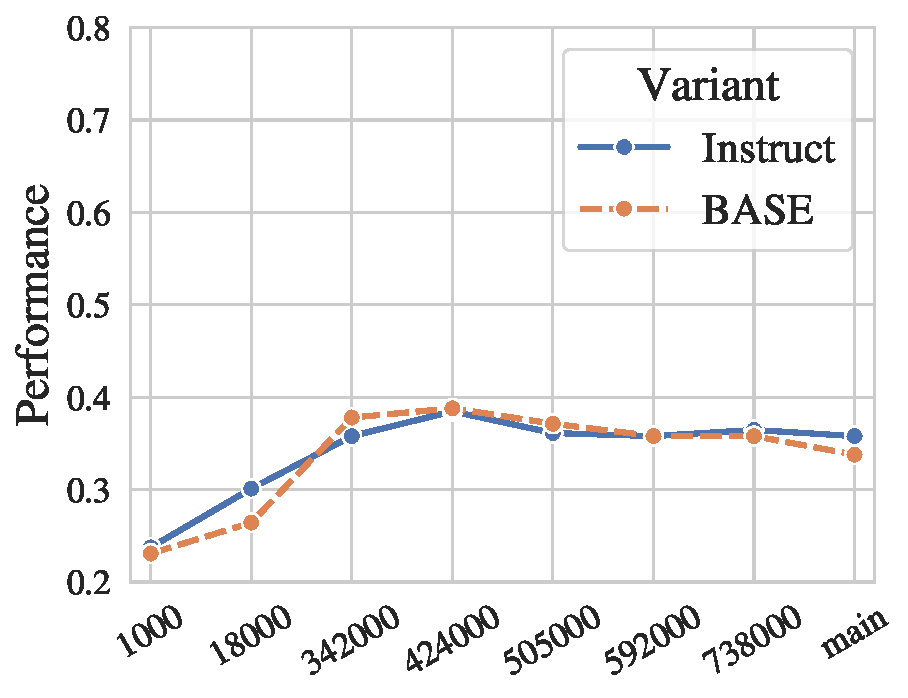
\includegraphics[width=\the\columnwidth]{figures/fig_files/it_ckpts/it_evalarc_challenge.pdf}
        \caption{ARC Challenge}
    \end{subfigure}%
    ~ 
    \begin{subfigure}[b]{0.3\textwidth}
    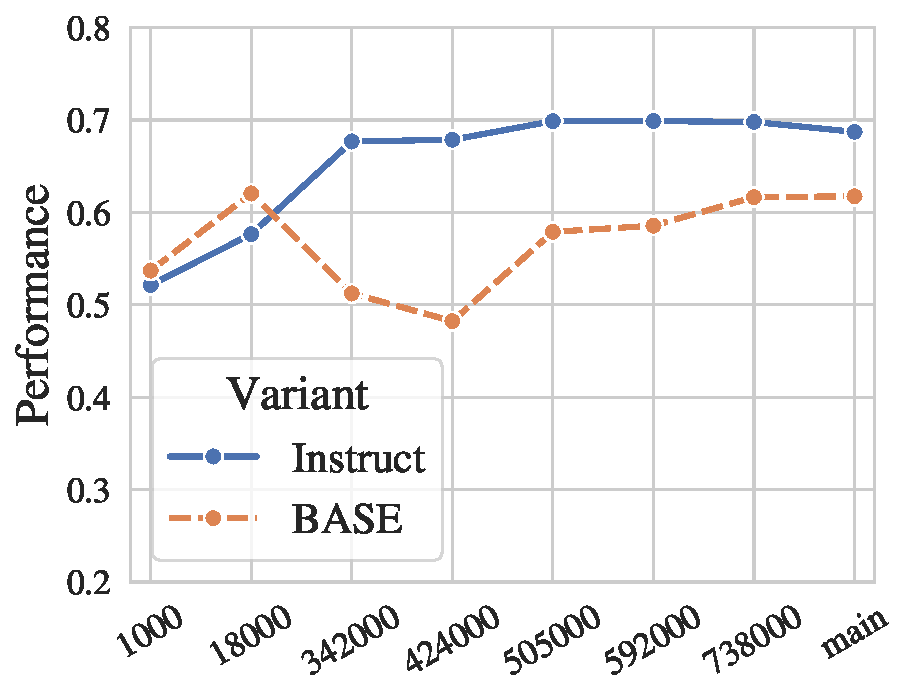
\includegraphics[width=\the\columnwidth]{figures/fig_files/it_ckpts/it_evalboolq.pdf}
        \caption{BoolQ}
    \end{subfigure}%
    \\
    \begin{subfigure}[b]{0.3\textwidth}
    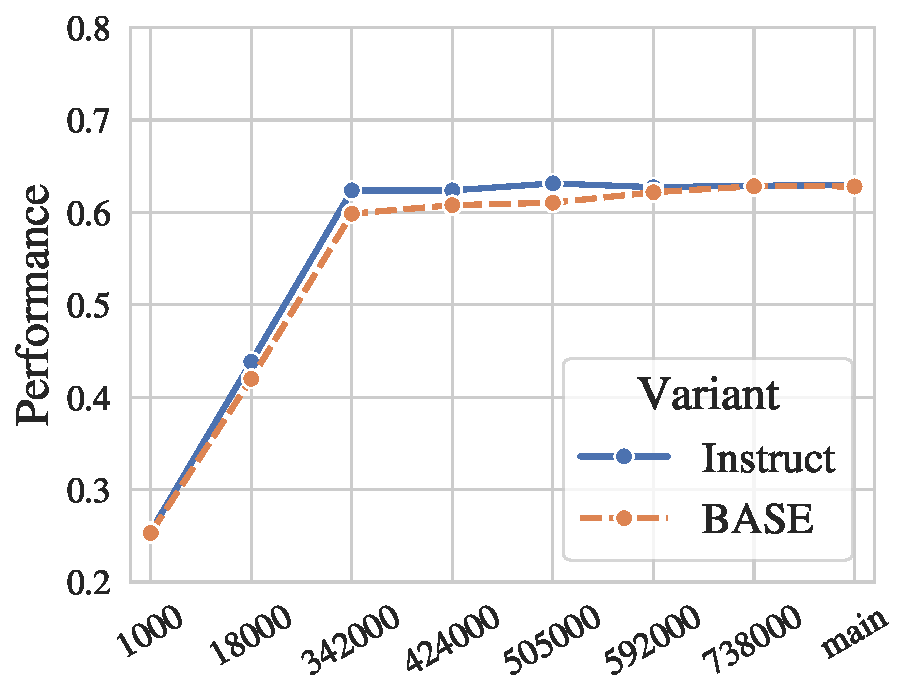
\includegraphics[width=\the\columnwidth]{figures/fig_files/it_ckpts/it_evalhellaswag.pdf}
        \caption{Hellaswag}
    \end{subfigure}%
    ~ 
    \begin{subfigure}[b]{0.3\textwidth}
    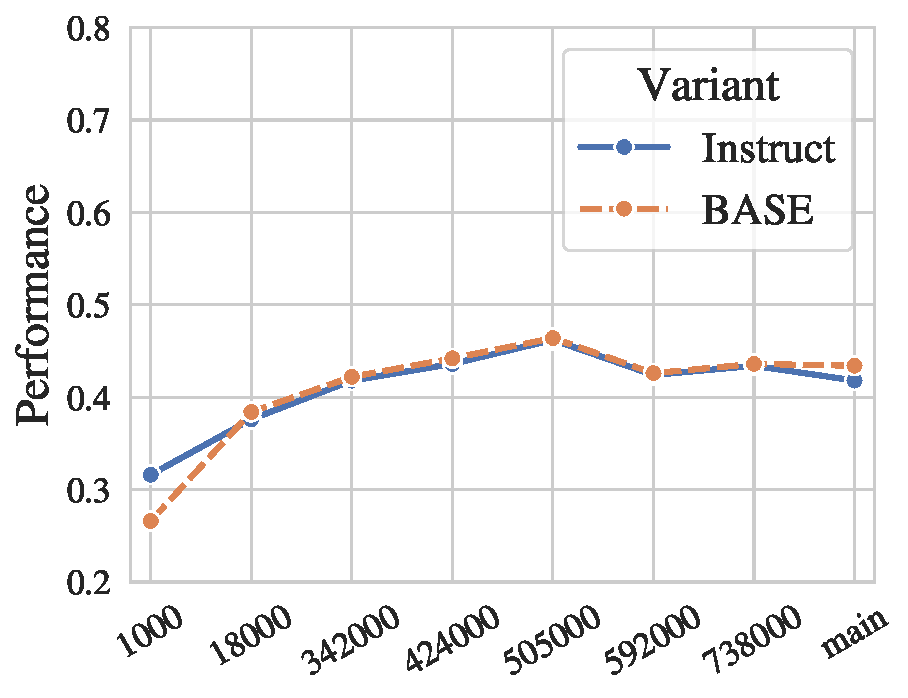
\includegraphics[width=\the\columnwidth]{figures/fig_files/it_ckpts/it_evalopenbookqa.pdf}
        \caption{Openbook QA}
    \end{subfigure}%
    ~ 
    \begin{subfigure}[b]{0.3\textwidth}
    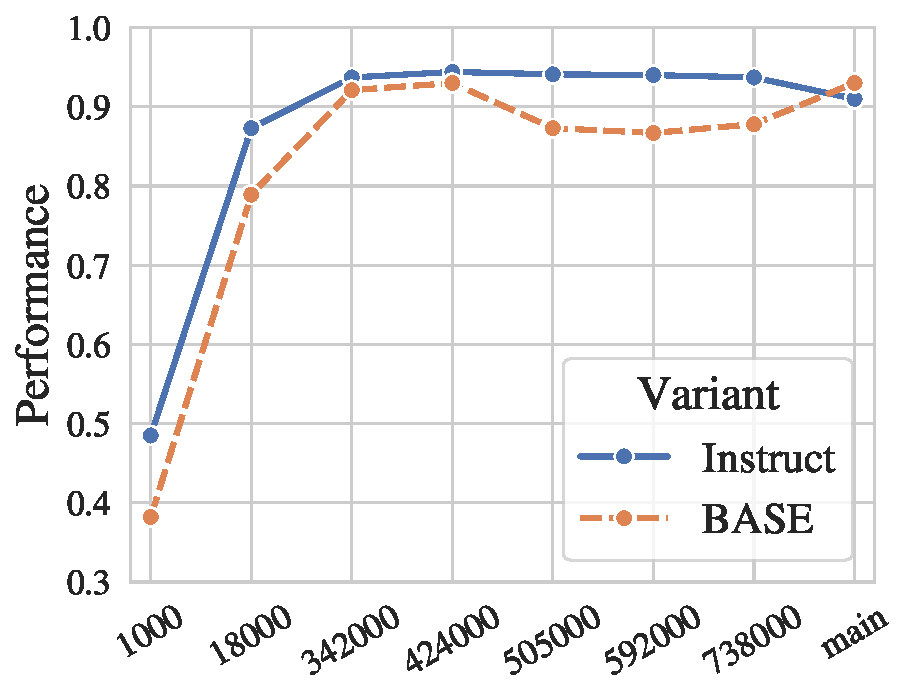
\includegraphics[width=\the\columnwidth]{figures/fig_files/it_ckpts/it_evalsciq.pdf}
        \caption{SciQ}
    \end{subfigure}%
    \caption{Model performance after instruction tuning on each pre-training step.}
    \label{fig:it-ckpt-perf}
\end{figure*}